\documentclass[11pt,a4paper]{article}
\usepackage[utf8]{inputenc}
\usepackage[german]{babel}
\usepackage[T1]{fontenc}
\usepackage{amsmath}
\usepackage{amsfonts}
\usepackage{amssymb}
\usepackage{graphicx}
\usepackage[margin=1.25cm]{geometry} % Puts the same margin on all borders of the document

% Packages

\usepackage{hyperref} % Generate hyperlinks to referenced items
\usepackage{adjustbox} % Used to change parameters in \includegraphics[scale=•]{•}
\usepackage{enumitem} % Provides several options for lists
\usepackage{verbatim} % Package to use \begin{comment}
\usepackage{pdfpages} % Used to import PDF pages
\usepackage{multirow} % Allows us to have a single cell in a table span multiple rows
\usepackage{makecell} % Allows us to format multiple lines in a single cell
\usepackage{minted} % Used to syntax highlight code
\usepackage{xcolor}  % Gives access to coloring text
\usepackage{longtable} % Allows us to create a table over multiple pages
\usepackage{float} % Improved placement of floating items
\usepackage{pdfpages} % Used to import pdf pages
\usepackage{booktabs} % Used for horizontal lines instead of \hline



% Settings

\graphicspath{{./files/}} % Sets path for files to the files folder in the same directory

\hypersetup{
    colorlinks=false, %set true if you want colored links
    linktoc=all,     %set to all if you want both sections and subsections linked
    linkcolor=blue,  %choose some color if you want links to stand out
}


\renewcommand{\arraystretch}{1.75} 

\lstset {
	literate={~} {$\sim$}{1},
    language=Java,
    basicstyle=\footnotesize,
    numbers=left,
    stepnumber=1,
    showstringspaces=false,
    tabsize=1,
    breaklines=true,
    breakatwhitespace=false,
    inputencoding=utf8,
    extendedchars=true   
}

\begin{titlepage}
  \title{FOP Reference Sheet} % document_name-type_of_document
  \author{Jonas Milkovits}
  \date{Last Edited: \today}
\end{titlepage}

\begin{document}

\pagenumbering{gobble}
\maketitle
\pagenumbering{roman} % i, ii, iii on beginning pages, that don't have content
\tableofcontents
\clearpage
\pagenumbering{arabic} % 1,2,3 on content pages

\begin{comment}
	\begin{tabular}{ | p{4cm} p{13.5cm} | }
	\hline
	\makecell[l]{} & \makecell[l]{$\rhd$  } \\ \hline
	
	\makecell[l]{} & \makecell[l]{$\rhd$  } \\ \hline
	
	\makecell[l]{} & \makecell[l]{$\rhd$  } \\ \hline
	
	\makecell[l]{} & \makecell[l]{$\rhd$  } \\ \hline
	
	\makecell[l]{} & \makecell[l]{$\rhd$  } \\ \hline
	
	\makecell[l]{} & \makecell[l]{$\rhd$  } \\ \hline
	
	\makecell[l]{} & \makecell[l]{$\rhd$  } \\ \hline
	
	\makecell[l]{} & \makecell[l]{$\rhd$  } \\ \hline
	\end{tabular}
\end{comment}


\section{Computerspeicher}



	\begin{tabular}{ | p{4cm} p{13.5cm} | }
	\hline
	\makecell[l]{Unsere Vorstellung} & 
	\makecell[l]{$\rhd$ großes Feld aus Maschinenwörtern mit eindeutiger Adresse} \\ \hline
	
	\makecell[l]{Erzeugung eines \\ neuen Objekts} & 
	\makecell[l]{$\rhd$ Reservierung von ungenutztem Speicher in ausreichender Größe} \\ \hline
	
	\makecell[l]{Referenz} & 
	\makecell[l]{$\rhd$ Name der Variable, die die Anfangsadresse des Objekts speichert \\ 
	$\rhd$ Kann auch an komplett anderer Stelle als das Objekt gespeichert sein } \\ \hline
	
	\makecell[l]{Speicherort primitiver \\ Datentypen} & 
	\makecell[l]{$\rhd$ Name verweist tatsächlich auf Speicherstelle, an der Wert abgespeichet wird } \\ \hline
	
	\makecell[l]{Prozessablauf} & 
	\makecell[l]{$\rhd$ Program Counter enthält Adresse der nächsten Anweisung \\
	\hspace{0.35cm} $\Rightarrow$ Zählt nach jeder Anwendung hoch und verweist auf nächsten Speicher \\
	$\rhd$ CPU verarbeitet parallel die momentane Anweisung aus Program Counter} \\ \hline
	
	\makecell[l]{Methodenausführung} & 
	\makecell[l]{$\rhd$ Einrichtung einer Variable \texttt{StackPointer} bei Programmstart \\
	$\rhd$ StackPointer enthält die Adresse des \texttt{Call-Stacks} \\
	$\rhd$ Bei Methodenaufruf wird im Speicher Platz reserviert, genannt \texttt{Frame} \\
	$\rhd$ \texttt{Frame}  wird dann auf dem Call-Stack abgelegt\\
	$\rhd$ Der \texttt{StackPointer}  wird dann mit der Adresse des neuen\texttt{Frames}  überschrieben \\
	$\rhd$ Methodenaufruf vorbei: Frame wird wieder vom \texttt{Call-Stack} genommen \\
	$\rhd$ \texttt{StackPointer} wird auf Adresse des vorherigen \texttt{Frames}  gesetzt} \\ \hline
	
	\makecell[l]{Methodentabelle} & \makecell[l]{$\rhd$ Enthält bei Objekt die Anfangsadressen der 
	verfügbaren Methoden } \\ \hline
	
	\end{tabular}
	
	\begin{center}
	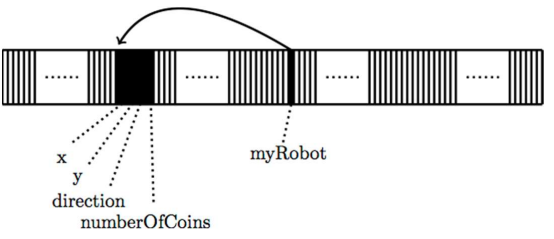
\includegraphics[scale=0.8]{computerspeicher}
	\end{center}

\section{Datenstrukturen}

\begin{tabular}{ | p{4cm} p{13.5cm} | }
	\hline
	\makecell[l]{Array} & 
	\makecell[l]{$\rhd$ Verwendet zum Speichern von mehreren Variablen des selben Typs \\
	$\rhd$ Erzeugung: \texttt{int[] test = new int[n];} \\
	$\rhd$ \texttt{n} gibt in diesem Fall die feste Anzahl der speicherbaren Variablen an \\
	$\rhd$ Natürlich auch Arrays von Objekten möglich \\
	$\rhd$ Zugriff auf Variablen: \texttt{test[0]} für ersten Wert (Index) \\
	$\rhd$ Zugriff auf Länge: \texttt{test.length} } \\ \hline
	\end{tabular}



\section{Datentypen}

	\begin{tabular}{ | p{4cm} p{13.5cm} | }
	\hline
	\makecell[l]{Konstanten} & \makecell[l]{$\rhd$ Variable/Referenz wird dadurch unveränderbar \\
	$\rhd$ z.B.: \texttt{final myClass ABC = new myClass();} \\
	\hspace{0.4cm} $\Rightarrow$ Referenz zwar nicht veränderbar, Objekt aber schon \\ 
	$\rhd$ \texttt{Integer.MAX\_VALUE / Integer.MIN\_VALUE} \\
	$\rhd$ Unendlich: \texttt{Double.POSITIVE\_INFINITY / Double.NEGATIVE\_INFINITY} } \\ \hline
	
	\makecell[l]{Primitive Dateitypen} & 
	\makecell[l]{$\rhd$ Ganze Zahlen: byte $\rightarrow$ short $\rightarrow$ int $\rightarrow$ long \\
	$\rhd$ Gebrochene Zahlen: float $\rightarrow$ double \\
	$\rhd$ Logik: boolean \\
	$\rhd$ Zeichen: char } \\ \hline
	
	\makecell[l]{Literale} & \makecell[l]{$\rhd$ wörtlich hingeschriebene Werte eines Datentyps  \\
	$\rhd$ Zahlen standardmäßig int, falls \texttt{long} gewünscht: \texttt{123L oder 123l} \\ 
	$\rhd$ Bei gebrochenen double, falls \texttt{float} gewünscht: \texttt{12.3F oder 12.3f} \\
	$\rhd$ null: Nutzung für Referenzen $\rightarrow$ verweist auf nichts} \\ \hline
	
	\makecell[l]{Boolean} & \makecell[l]{$\rhd$ nur \texttt{true} und \texttt{false} \\
	$\rhd$ Negation \texttt{!a} \\
	$\rhd$ Logisches Und: \texttt{a \&\& b} \\
	$\rhd$ Logisches Oder: \texttt{a || b} (inklusiv) \\
	$\rhd$ Gleichheit: \texttt{a == b} } \\ \hline
	
	\makecell[l]{Zeichentyp char} & \makecell[l]{$\rhd$ z.B.: \texttt{char c = ´a´;} \\
	$\rhd$ Interne Kodierung als Unicode \\
	$\rhd$ ´$\textbackslash$t´ Horizontaler Tab \\
	$\rhd$ ´$\textbackslash$b´ Backspace \\
	$\rhd$ ´$\textbackslash$n´ Neue Zeile \\
	$\rhd$ Auch Darstellung im Hexacode (´$\textbackslash$u039A´)} \\ \hline
	
	\makecell[l]{Enumeration} & \makecell[l]{$\rhd$ Zusammenfassung mehrerer Konstanten (feste Anzahl)\\
	$\rhd$ Erzeugung meist in eigener .java Datei \\
	$\rhd$ \texttt{enum MyDirection \{DOWN, RIGHT\} } \\
	$\rhd$ Keine Objekterzeugung von Enumeration möglich \\
	$\rhd$ Abspeichern in Variable des Enum-Types ist jedoch möglich \\
	$\rhd$ \texttt{MyDirection dir = MyDirection.DOWN;} } \\ \hline
	\end{tabular}

\section{Interfaces}
	\begin{tabular}{ | p{4cm} p{13.5cm} | }
	\hline
	\makecell[l]{Erzeugung} & \makecell[l]{$\rhd$ Meist in eigener Datei \\
	$\rhd$ \texttt{public interface MyInterface \{...\}} \\
	$\rhd$ Alle Methodes und das Interface \textbf{müssen} \texttt{public} sein \\ } \\ \hline
	
	\makecell[l]{Methoden} & 
	\makecell[l]{$\rhd$ Werden hier nicht implementiert, sondern nur definiert \\
	$\rhd$ \texttt{public} kann weggelassen werden, da ohnehin notwending } \\ \hline
	
	\makecell[l]{Verwendung} & \makecell[l]{$\rhd$ \texttt{implements MyInterface} nach Klassenname } \\ \hline
	
	\makecell[l]{} & \makecell[l]{$\rhd$  } \\ \hline
	
	\makecell[l]{} & \makecell[l]{$\rhd$  } \\ \hline
	
	\makecell[l]{} & \makecell[l]{$\rhd$  } \\ \hline
	
	\makecell[l]{} & \makecell[l]{$\rhd$  } \\ \hline
	
	\makecell[l]{} & \makecell[l]{$\rhd$  } \\ \hline
	\end{tabular}



\section{Klassen}

	\begin{tabular}{ | p{4cm} p{13.5cm} | }
	\hline
	\makecell[l]{Erzeugung} & \makecell[l]{$\rhd$ meist in seperater .java Datei  \\
	$\rhd$ \texttt{public class MyClass \{\}} } \\ \hline
	
	\makecell[l]{Attribute} & \makecell[l]{$\rhd$ Eigenschaften der Objekte/Klassen \\
	$\rhd$ z.B.: \texttt{private int x;} (Objekteigenschaft) \\
	$\rhd$ z.B.: \texttt{private static int x;} (Klasseneigenschaft)  } \\ \hline
	
	\makecell[l]{Konstruktor} & 
	\makecell[l]{$\rhd$ Wird zur Erzeugung von neuen Objekten einer Klasse verwendet \\
	$\rhd$ Methode mit selben Namen wie Klasse und ohne Rückgabetyp \\
	$\rhd$ z.B.: \texttt{public MyClass (int x, int y) \{this.x = x; this.y = y;\}} \\
	$\rhd$ Erzeugung eines neuen Objekts: \texttt{MyClass test = new MyClass(2,4);} \\
	$\rhd$ Falls kein Konstruktur angegeben wird $\rightarrow$ Standardkonstruktor } \\ \hline

	\end{tabular}

\section{Konversionen}

	\begin{tabular}{ | p{4cm} p{13.5cm} | }
	\hline
	\makecell[l]{Implizit} & 
	\makecell[l]{$\rhd$ Immer möglich, wenn kein Informationsverlust entstehen kann \\
	$\rhd$ z.B.: kleinerer Datentyp in größeren } \\ \hline
	
	\makecell[l]{Explizit} & \makecell[l]{$\rhd$ Meist Informationsverlust \\
	$\rhd$ Durchführung durch Angabe des Datentyps in Klammern davor \\
	$\rhd$ z.B.: \texttt{int i = (int)testDouble;} } \\ \hline
	\end{tabular}


\section{Methoden}
	\begin{tabular}{ | p{4cm} p{13.5cm} | }
	\hline
	\makecell[l]{Methodenkopf} & 
	\makecell[l]{$\rhd$  Modifier Rückgabewert Methodenname (Parameter) \{Anweisung\} \\
	$\rhd$ z.B.: \texttt{public void setX (int x) \{this.x = x;\}} (Objektmethode) \\
	$\rhd$ z.B.: \texttt{public static void setY (int y) \{this.y = y;\}} (Klassenmethode) \\
	$\rhd$ \texttt{this.x} steht hier für das Objektattribut und nicht den Parameter} \\ \hline
	
	\makecell[l]{Ausführung} & \makecell[l]{$\rhd$ Objektmethoden: \texttt{myObject.setX(2);} \\
	$\rhd$ Klassenmethoden: \texttt{MyClass.setY(2);}} \\ \hline
	
	\makecell[l]{return} & 
	\makecell[l]{$\rhd$ Wird für Rückgabe bei Methoden mit Rückgabewert benötigt } \\ \hline
	\end{tabular}

\section{Packages und Zugriffsrechte}
	\begin{tabular}{ | p{4cm} p{13.5cm} | }
	\hline
	\makecell[l]{Packages} & \makecell[l]{$\rhd$ Zusammenfassung von mehreren Dateien \\
	$\rhd$ \texttt{import package.*;} \\
	$\rhd$ \texttt{*} steht für alle Definitionen aus \texttt{package} \\
	$\rhd$ Import-Anweisungen müssen immer am Anfang des Quelltextes stehen } \\ \hline
	
	\makecell[l]{Zugriffsrechte} & \makecell[l]{$\rhd$ Klassen/Enum: nur \texttt{public} oder nichts \\
	\hspace{0.4cm} $\Rightarrow$ Nur eine Klasse darf \texttt{public} sein (Damit auch Dateiname) \\
	$\rhd$ \texttt{private:} Zugriff innerhalb der Klasse \\
	$\rhd$ \texttt{Keine Angabe:} \texttt{private} + im Package \\
	$\rhd$ \texttt{protected:} \texttt{Keine Angabe} + in allen Subklassen \\
	$\rhd$ \texttt{public:} \texttt{protected} + an jeder Import-Stelle } \\ \hline
	\end{tabular}


\section{Programme und Prozesse}

	\begin{tabular}{ | p{4cm} p{13.5cm} | }
	\hline
	\makecell[l]{Quelltest} & \makecell[l]{$\rhd$ z.B. selbst geschriebener Java-Code } \\ \hline
	
	\makecell[l]{Java-Bytecode} & \makecell[l]{$\rhd$ Wird durch Übersetzung des Java-Quelltextes erzeugt } \\ \hline
	
	\makecell[l]{Programm} & \makecell[l]{$\rhd$ Sequenz von Informationen} \\ \hline
		
	\makecell[l]{Aufruf eines Programms} & \makecell[l]{$\rhd$ Starten eines Prozesses, 
	der die Anweisungen des	Programmes abarbeitet } \\ \hline
	
	\makecell[l]{Prozesse} & \makecell[l]{$\rhd$ CPU besteht aus mehreren Prozessorkernen \\
	$\rhd$ Mehrere Prozesse laufen dementsprechend parallel \\
	$\rhd$ Allerdings bearbeitet jeder Kern nur einen Prozess gleichzeitig (sehr kurz) \\
	\hspace{0.4cm}$\Rightarrow$ Illusion von Multitasking } \\ \hline
	
	\makecell[l]{} & \makecell[l]{$\rhd$  } \\ \hline
	\end{tabular}
	
\section{Schleifen und if}

	\begin{tabular}{ | p{4cm} p{13.5cm} | }
	\hline
	\makecell[l]{while-Schleife} & \makecell[l]{$\rhd$ \texttt{while (Bedingung) \{Anweisung;\}} \\ 
	$\rhd$ Schleife wird ausgeführt, solange die Bedingung wahr ist \\ 
	$\rhd$ \{\} kann bei einzelner Anweisung auch weggelassen werden } \\ \hline
	
	\makecell[l]{do-while-Schleife} & 
	\makecell[l]{$\rhd$ \texttt{do \{Anweisung;\} while (Bedingung);} \\ 
	$\rhd$ Anweisungsblock wird immer mindestens einmal ausgeführt } \\ \hline
	
	\makecell[l]{for-Schleife} & 
	\makecell[l]{$\rhd$ \texttt{for (Anweisung davor; Bedingung; Anweisung danach) \{Anweisung\}} \\
	$\rhd$ z.B.: \texttt{for (int i = 0; i < 10; i++) \{...\}} \\
	\hspace{0.4cm}$\Rightarrow$ Zehnmalige Ausführung der Anweisung \\
	$\rhd$ Kurzform: \texttt{for (Position p : positions) \{\}}} \\ \hline
	
	\makecell[l]{if-Anweisung} & \makecell[l]{$\rhd$ \texttt{if (Bedingung) \{...\}} \\
	\hspace{0.4cm} $\rhd$ Führt den Code in der Anweisung nur aus, falls die Bedingung erfüllt ist \\
	$\rhd$ \texttt{if (Bedingung) \{\} else \{\}} \\
	\hspace{0.4cm} $\rhd$ Code, der ausgeführt wird, falls Bedingung nicht erfüllt ist} \\ \hline
	\end{tabular}
	
	
\section{Syntax}

	\begin{tabular}{ | p{4cm} p{13.5cm} | }
	\hline
	\makecell[l]{Keywords} & \makecell[l]{$\rhd$ Können nur an bestimmten Stellen im Code stehen \\
	$\rhd$ z.B. \texttt{class, import, public, while,..}} \\ \hline
	
	\makecell[l]{Identifier} & \makecell[l]{$\rhd$ Namen für Klassen, Variablen, Methoden,.. \\
	$\rhd$ Erstes Zeichen darf keine Ziffer sein \\
	$\rhd$ Keine Keywords als Identifier
	$\rhd$ Identifier sind case-sensitive } \\ \hline
	
	\makecell[l]{Konventionen} & \makecell[l]{
	$\rhd$ Variablen / Methoden beginnen mit Kleinbuchstaben (\texttt{testInt}) \\
	$\rhd$ Klassen beginnen mit Großbuchstaben (\texttt{testClass}) \\
	$\rhd$ Wortanfänge im Inneren mit Großbuchstaben \\
	$\rhd$ Konstanten bestehen aus $\_$ und Großbuchstaben (\texttt{CENTS$\_$PER$\_$EURO})} \\ \hline
	
	\makecell[l]{Kommentare} & \makecell[l]{$\rhd$ \texttt{//} Einzelne Zeile \\
	$\rhd$ \texttt{/*...*/} Mehrere Zeilen \\
	$\rhd$ \texttt{/**...*/} Erzeugung von Javadoc }  \\ \hline
	\end{tabular}
	
\section{Vererbung}
	\begin{tabular}{ | p{4cm} p{13.5cm} | }
	\hline
	\makecell[l]{Zweck} & \makecell[l]{$\rhd$ Weitergabe von allen Methoden und Attributen } \\ \hline
	
	\makecell[l]{Verwendung} & 
	\makecell[l]{$\rhd$ \texttt{public class MySubClass extends MyClass \{\}} } \\ \hline
	
	\makecell[l]{Konstruktor} & 
	\makecell[l]{$\rhd$ Aufruf des Konstruktors der Superklasse mithilfe von \texttt{super(Parameter);} \\
	$\rhd$ Dieser Aufruf erfolgt im Konstruktor der Subklasse \\
	$\rhd$ z.B.: \texttt{public MySubClass (int x) \{ super(x);<v\}}} \\ \hline
	
	\makecell[l]{Overwrite} & \makecell[l]{$\rhd$ Methoden in Subklassen können auch neu geschrieben werden \\
	\hspace{0.4cm} $\Rightarrow$ Die Implementation der Superklasse wird sozusagen überschrieben \\
	$\rhd$ Selber Name und Parameterliste notwendig } \\ \hline
	
	\makecell[l]{Overload} & 
	\makecell[l]{$\rhd$ Methoden mit selbem Bezeichner, aber unterschiedlicher Parameterliste \\
	$\rhd$ Die Methode wird überladen \\ 
	$\rhd$ Konstruktoren kann man auch überladen \\
	\hspace{0.4cm} $\Rightarrow$ Für manche Werte werden dann Standardwerte gesetzt \\
	\hspace{0.4cm} $\Rightarrow$ Anderer Konstruktor auch in Konstruktor aufrufbar 
	(\texttt{this(1);}) } \\ \hline
	
	\makecell[l]{} & \makecell[l]{$\rhd$  } \\ \hline
	
	\makecell[l]{} & \makecell[l]{$\rhd$  } \\ \hline
	
	\makecell[l]{} & \makecell[l]{$\rhd$  } \\ \hline
	\end{tabular}


\end{document}